%**************************************************************************************
% Neural Networks and Function Approximation - COMPREHENSIVE REORGANIZED VERSION
% All content from original preserved, just reorganized according to reorganized_presentation.md
%**************************************************************************************

\documentclass[aspectratio=169]{beamer}

\mode<presentation> {
	\usetheme{Madrid}
	
	% Burnt orange
	\definecolor{burntorange}{rgb}{0.8, 0.33, 0.0}
	\colorlet{beamer@blendedblue}{burntorange}
	% Pale yellow
	\definecolor{paleyellow}{rgb}{1.0, 1.0, 0.953}
	\setbeamercolor{background canvas}{bg=paleyellow}
	% Secondary and tertiary palette
	\setbeamercolor*{palette secondary}{use=structure,fg=white,bg=burntorange!80!black}
	\setbeamercolor*{palette tertiary}{use=structure,fg=white,bg=burntorange!60!black}
	
	% Remove navigation symbols
	\setbeamertemplate{navigation symbols}{}
}

\usepackage{amsmath,amssymb,amsthm}
\usepackage{bm}
\usepackage{booktabs}
\usepackage{graphicx}
\usepackage[labelsep=space,tableposition=top]{caption}
\renewcommand{\figurename}{Fig.} 
\usepackage{caption,subcaption}
\usepackage{xcolor}
\usepackage{transparent}
\usepackage{hyperref}
\usepackage{tikz}
\usepackage{listings}
\usepackage{algorithm}
\usepackage{algorithmic}
\usetikzlibrary{shapes,arrows,positioning,calc}
\usepackage{pgfplots}
\pgfplotsset{compat=1.17}

% Define math operators
\DeclareMathOperator*{\argmin}{arg\,min}
\DeclareMathOperator*{\argmax}{arg\,max}
\DeclareMathOperator{\ReLU}{ReLU}
\DeclareMathOperator{\sign}{sign}
\newcommand{\norm}[1]{\left\lVert#1\right\rVert}

% Code listing style
\lstset{
    language=Python,
    basicstyle=\tiny\ttfamily,
    keywordstyle=\color{blue},
    commentstyle=\color{gray},
    stringstyle=\color{green!70!black},
    showstringspaces=false,
    frame=single,
    breaklines=true,
    numbers=left,
    numberstyle=\tiny
}

%----------------------------------------------------------------------------------------
%	TITLE PAGE
%----------------------------------------------------------------------------------------
\title[Neural Networks \& Function Approximation]{Neural Networks and Function Approximation} 
\subtitle{Multi-Layer Perceptrons in Scientific Machine Learning}
\author{Krishna Kumar}
\institute[UT Austin]{
	University of Texas at Austin \\
	\medskip
	\textit{\url{krishnak@utexas.edu}}
}
\date{}

\begin{document}

\begin{frame}
\titlepage
\end{frame}

\begin{frame}{Outline}
\tableofcontents
\end{frame}

%========================================================================================
% PART I: MOTIVATION AND PROBLEM SETUP
%========================================================================================
\section{Part I: Motivation and Problem Setup}

\begin{frame}{The Central Challenge}
\begin{block}{Core Question}
Can we build a machine that learns to approximate any continuous function from data?
\end{block}

\vspace{0.5em}

\textbf{Applications in Scientific Machine Learning:}
\begin{itemize}
    \item Solving partial differential equations (PDEs) without meshes
    \item Learning constitutive models from experimental data
    \item Discovering governing equations from observations
    \item Building surrogate models for optimization
    \item Uncertainty quantification in complex systems
\end{itemize}

\vspace{0.5em}

\textbf{What we'll explore:}
\begin{itemize}
    \item Mathematical foundations (Weierstrass → Universal Approximation)
    \item Building blocks (perceptron → deep networks)
    \item Training algorithms (gradient descent → backpropagation)
    \item Practical considerations (architecture, regularization)
\end{itemize}
\end{frame}

\begin{frame}{The Benchmark Problem: 1D Poisson Equation}
\begin{columns}
\column{0.5\textwidth}
\textbf{Problem formulation:}
\begin{equation}
\begin{cases}
-\nabla^2 u = f & \text{in } \Omega \\
u = g & \text{on } \partial\Omega
\end{cases}
\end{equation}

\textbf{1D case:}
$$-\frac{d^2u}{dx^2} = f(x), \quad u(0) = u(1) = 0$$
For the source term $f(x) = \pi^2 \sin(\pi x)$

\textbf{Analytical solution:} $u(x) = \sin(\pi x)$

\column{0.5\textwidth}
\begin{figure}
\centering
\includegraphics[width=\textwidth]{figs/poisson-analytical-solution.png}
\caption{Analytical solution showing parabolic profile}
\end{figure}
\end{columns}

\vspace{0.3cm}
\textbf{Challenge:} Can we learn this solution from sparse, noisy measurements?
\end{frame}

\begin{frame}{The Function Approximation Challenge}
\begin{figure}
\centering
\includegraphics[width=0.6\textwidth]{figs/sparse-data-challenge.png}
\caption{Learning from sparse data: 15 noisy measurements to reconstruct continuous solution}
\end{figure}

\end{frame}

\begin{frame}{The Function Approximation Challenge}
\begin{columns}
\column{0.5\textwidth}
\textbf{Given:}
\begin{itemize}
    \item Sparse measurements (e.g., 15 points)
    \item Noisy observations
    \item Unknown functional form
    \item Potentially high dimensions
\end{itemize}

\column{0.5\textwidth}
\textbf{Goal:}
\begin{itemize}
    \item Reconstruct continuous solution
    \item Quantify uncertainty
    \item Generalize to new domains
    \item Handle complex geometries
\end{itemize}
\end{columns}
\end{frame}

\begin{frame}{Traditional Methods: Finite Differences}
\begin{columns}
\column{0.45\textwidth}
\begin{figure}
\centering
\includegraphics[width=\textwidth]{figs/finite-difference-methods.png}
\caption{Finite difference discretization}
\end{figure}

\column{0.55\textwidth}
\textbf{The approach:}
\begin{itemize}
    \item Discretize domain into grid
    \item Approximate derivatives: \\
    $\frac{d^2u}{dx^2} \approx \frac{u_{i+1} - 2u_i + u_{i-1}}{h^2}$
    \item Solve linear system: $Au = b$
\end{itemize}

\textbf{Limitations:}
\begin{itemize}
    \item Fixed grid resolution
    \item Curse of dimensionality ($O(N^d)$)
    \item Poor for irregular domains
    \item Cannot learn from data
    \item No continuous representation
\end{itemize}
\end{columns}
\end{frame}

\begin{frame}{Finite Difference Results}
\begin{figure}
\centering
\includegraphics[width=0.8\textwidth]{figs/fd-poisson.png}
\caption{Finite difference solution: accurate but discrete, requires mesh}
\end{figure}

\textbf{Key observation:} We need a flexible, continuous, learnable representation
\end{frame}

%========================================================================================
% PART II: MATHEMATICAL FOUNDATIONS
%========================================================================================
\section{Part II: Mathematical Foundations}

\begin{frame}{Historical Perspective: From Polynomials to Neural Networks}
\begin{center}
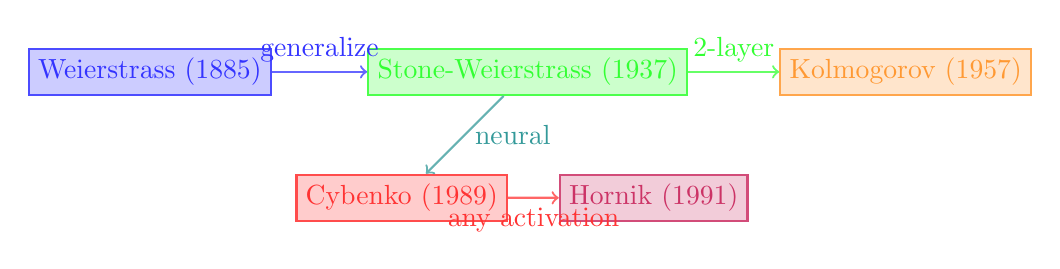
\begin{tikzpicture}[scale=0.8]
	\node[draw=blue!70, rectangle, fill=blue!20, text=blue!80, thick] (w) at (-2,0) {Weierstrass (1885)};
	\node[draw=green!70, rectangle, fill=green!20, text=green!80, thick] (s) at (4,0) {Stone-Weierstrass (1937)};
	\node[draw=orange!70, rectangle, fill=orange!20, text=orange!80, thick] (k) at (10,0) {Kolmogorov (1957)};
	\node[draw=red!70, rectangle, fill=red!20, text=red!80, thick] (c) at (2,-2) {Cybenko (1989)};
	\node[draw=purple!70, rectangle, fill=purple!20, text=purple!80, thick] (h) at (6,-2) {Hornik (1991)};
	
	\draw[->, thick, color=blue!60] (w) -- (s) node[midway,above,color=blue!80] {generalize};
	\draw[->, thick, color=green!60] (s) -- (k) node[midway,above,color=green!80] {2-layer};
	\draw[->, thick, color=teal!60] (s) -- (c) node[midway,right,color=teal!80] {neural};
	\draw[->, thick, color=red!60] (c) -- (h) node[midway,below,color=red!80] {any activation};
\end{tikzpicture}
\end{center}

\vspace{0.5cm}

\begin{itemize}
    \item \textbf{Weierstrass (1885):} Polynomials can approximate continuous functions
    \item \textbf{Stone-Weierstrass (1937):} Generalization to abstract spaces
    \item \textbf{Kolmogorov (1957):} 2-layer networks suffice
    \item \textbf{Cybenko (1989):} Sigmoid networks are universal
    \item \textbf{Hornik (1991):} Any non-polynomial activation works
\end{itemize}
\end{frame}

\begin{frame}{The Weierstrass Approximation Theorem}
\begin{block}{Theorem (Weierstrass, 1885)}
For any continuous function $f: [a,b] \to \mathbb{R}$ and any $\epsilon > 0$, there exists a polynomial $P(x)$ such that:
$$|f(x) - P(x)| < \epsilon \quad \forall x \in [a,b]$$
\end{block}

\vspace{0.5cm}

\textbf{Interpretation:}
\begin{itemize}
    \item Continuous functions can be uniformly approximated by polynomials
    \item Approximation quality improves with polynomial degree
    \item Foundation for all approximation theory
\end{itemize}

\textbf{Constructive proof:} Bernstein polynomials
$$B_n[f](x) = \sum_{k=0}^{n} f\left(\frac{k}{n}\right) \binom{n}{k} x^k (1-x)^{n-k}$$
\end{frame}

\begin{frame}{Polynomial Approximation of sparse data}
	\begin{figure}
		\centering
		\includegraphics[width=\textwidth]{figs/polynomial-approx-sparse.png}
		\caption{Runge osciallations at higher degree polynomial. Max 14, ntrain - 1 data points}
	\end{figure}
\end{frame}

\begin{frame}{Polynomial Approximation in Action}
\begin{columns}
\column{0.65\textwidth}
\begin{figure}
    \centering
    \includegraphics[width=\textwidth]{figs/polynomial-approximation-sinpi.png}
    \caption{Polynomial approximation of $\sin(\pi x)$ with increasing degrees}
\end{figure}
\column{0.35\textwidth}
\textbf{Convergence:}
\begin{itemize}
    \item Degree 3: captures trend
    \item Degree 5: better fit
    \item Degree 7: good accuracy
    \item Degree 9: excellent
\end{itemize}

\textbf{But:}
\begin{itemize}
    \item Runge phenomenon
    \item Global basis functions
    \item Poor for discontinuities
\end{itemize}
\end{columns}
\end{frame}

\begin{frame}{Bernstein Polynomials: Constructive Proof}
\begin{columns}
\column{0.4\textwidth}
\textbf{Bernstein basis:}
$$B_{k,n}(x) = \binom{n}{k} x^k (1-x)^{n-k}$$

\textbf{Approximation:}
$$B_n[f](x) = \sum_{k=0}^{n} f\left(\frac{k}{n}\right) B_{k,n}(x)$$

\textbf{Properties:}
\begin{itemize}
    \item Non-negative
    \item Partition of unity
    \item Local control
    \item Uniform convergence
\end{itemize}

\column{0.6\textwidth}
\begin{figure}
    \centering
    \includegraphics[width=\textwidth]{figs/bernstein-approximation.png}
    \caption{Bernstein polynomial basis functions}
\end{figure}
\end{columns}
\end{frame}

\begin{frame}{Convergence Analysis}
\begin{columns}
\column{0.35\textwidth}
\textbf{Convergence rate:}
For $f \in C^n[0,1]$:
$$\|f - P_n\|_\infty = O(1/\sqrt{n})$$

\textbf{Smooth functions:}
Exponential convergence for analytic functions

\column{0.65\textwidth}
\begin{figure}
    \centering
    \includegraphics[width=\textwidth]{figs/polynomial-convergence.png}
    \caption{Exponential convergence for smooth functions}
\end{figure}
\end{columns}
\end{frame}

\begin{frame}{Polynomial vs Neural Network Comparison}
\begin{figure}
    \centering
    \includegraphics[width=0.9\textwidth]{figs/polynomial-vs-nn-comparison.png}
\end{figure}
\end{frame}

\begin{frame}{Polynomial vs Neural Network: Key differences}
\begin{columns}
\column{0.5\textwidth}
\textbf{Polynomials:}
\begin{itemize}
    \item Global basis functions
    \item Fixed structure
    \item Runge phenomenon [Oscillations at the boundaries]
    \item Poor for high dimensions
\end{itemize}

\column{0.5\textwidth}
\textbf{Neural Networks:}
\begin{itemize}
    \item Localized representations
    \item Adaptive placement
    \item Compositional structure
    \item Dimension-friendly
\end{itemize}
\end{columns}
\end{frame}

\begin{frame}{High-Frequency Functions: A Challenge}
\begin{columns}
\column{0.65\textwidth}
\begin{figure}
    \centering
    \includegraphics[width=\textwidth]{figs/high-freq-comparison.png}
    \caption{High-frequency function challenges}
\end{figure}
\column{0.35\textwidth}
\textbf{Problem:}
Approximating $\sin(100x)$

\textbf{Polynomials:}
\begin{itemize}
    \item Need degree $\sim 100$
    \item Numerical instability
    \item Runge phenomenon
\end{itemize}

\textbf{Neural Networks:}
\begin{itemize}
    \item Adaptive placement
    \item Local features
    \item Compositional
\end{itemize}
\end{columns}
\end{frame}

\begin{frame}{Universal Approximation Theorem}
\begin{block}{Theorem (Cybenko, 1989)}
Let $\sigma$ be a continuous, bounded, non-constant, monotonically increasing function. 
Then finite sums of the form:
$$G(x) = \sum_{i=1}^{N} \alpha_i \sigma(w_i^T x + b_i)$$
are dense in $C([0,1]^n)$ under the supremum norm.
\end{block}

\vspace{0.5cm}

\textbf{In plain English:}
A single hidden layer neural network can approximate any continuous function to arbitrary accuracy, given enough neurons.

\vspace{0.3cm}

\textbf{Key points:}
\begin{itemize}
    \item Existence guarantee, not constructive
    \item Says nothing about number of neurons needed
    \item Doesn't tell us how to find the weights
\end{itemize}
\end{frame}

\begin{frame}{UAT Visualization}
\begin{figure}
\centering
\includegraphics[width=0.8\textwidth]{figs/uat-approximation-progression.png}
\caption{Neural network approximation with increasing width: 2, 10, and 50 neurons}
\end{figure}

\textbf{Observations:}
\begin{itemize}
    \item More neurons → better approximation
    \item Each neuron adds a "bump" or feature
    \item Adaptive placement of features
    \item No fixed polynomial structure
\end{itemize}
\end{frame}

%========================================================================================
% PART III: BUILDING NEURAL NETWORKS
%========================================================================================
\section{Part III: Building Neural Networks}

\begin{frame}{The Perceptron: Building Block of Neural Networks}
\begin{columns}
\column{0.5\textwidth}
\textbf{Mathematical model:}
\begin{equation}
\hat{y} = \sigma(\mathbf{w}^T\mathbf{x} + b)
\end{equation}

where:
\begin{itemize}
    \item $\mathbf{x} \in \mathbb{R}^n$: input features
    \item $\mathbf{w} \in \mathbb{R}^n$: weights
    \item $b \in \mathbb{R}$: bias
    \item $\sigma(\cdot)$: activation function
    \item $\hat{y}$: output/prediction
\end{itemize}

\textbf{Geometric interpretation:}
\begin{itemize}
    \item Linear decision boundary
    \item Hyperplane: $\mathbf{w}^T\mathbf{x} + b = 0$
    \item Normal vector: $\mathbf{w}$
    \item Distance from origin: $|b|/\|\mathbf{w}\|$
\end{itemize}

\column{0.5\textwidth}
\begin{figure}
\centering
\includegraphics[width=\textwidth]{figs/perceptron.png}
\caption{Perceptron model: linear combination followed by activation}
\end{figure}
\end{columns}
\end{frame}

\begin{frame}[fragile]{Linear Perceptron Implementation}
\begin{lstlisting}[language=Python]
import numpy as np

class LinearPerceptron:
    def __init__(self, input_dim):
        # Initialize weights randomly
        self.w = np.random.randn(input_dim) * 0.01
        self.b = np.random.randn() * 0.01
    
    def forward(self, x):
        """Compute output for input x"""
        return np.dot(x, self.w) + self.b
    
    def sigmoid(self, z):
        """Sigmoid activation function"""
        return 1 / (1 + np.exp(-z))
    
    def predict(self, x):
        """Make binary prediction"""
        z = self.forward(x)
        return self.sigmoid(z) > 0.5
    
    def train(self, X, y, lr=0.01, epochs=100):
        """Train using gradient descent"""
        for epoch in range(epochs):
            # Forward pass
            z = self.forward(X)
            y_pred = self.sigmoid(z)
            
            # Compute loss (binary cross-entropy)
            loss = -np.mean(y * np.log(y_pred + 1e-8) + 
                           (1-y) * np.log(1-y_pred + 1e-8))
            
            # Backward pass (gradient computation)
            dz = y_pred - y
            dw = X.T @ dz / len(y)
            db = np.mean(dz)
            
            # Update parameters
            self.w -= lr * dw
            self.b -= lr * db
            
            if epoch % 10 == 0:
                print(f"Epoch {epoch}, Loss: {loss:.4f}")
\end{lstlisting}
\end{frame}

\begin{frame}{Training a Linear Model}
\begin{columns}
\column{0.5\textwidth}
\textbf{Gradient Descent:}
\begin{align}
\mathcal{L} &= \frac{1}{2}\sum_{i=1}^{n} (y_i - \hat{y}_i)^2 \\
\frac{\partial \mathcal{L}}{\partial w_j} &= -\sum_{i=1}^{n} (y_i - \hat{y}_i) x_{ij} \\
w_j &\leftarrow w_j - \eta \frac{\partial \mathcal{L}}{\partial w_j}
\end{align}

\textbf{Learning process:}
\begin{itemize}
    \item Start with random weights
    \item Compute predictions
    \item Calculate error
    \item Update weights in direction of negative gradient
    \item Repeat until convergence
\end{itemize}

\column{0.5\textwidth}
\begin{figure}
\centering
\includegraphics[width=\textwidth]{figs/sgd.png}
\caption{Gradient descent trajectory in weight space}
\end{figure}
\end{columns}
\end{frame}

\begin{frame}{Linear Models Work for Linearly Separable Data}
\begin{figure}
\centering
% Linear separable figure not available
\includegraphics[width=0.8\textwidth]{figs/perceptron.png}
\caption{Linear perceptron successfully classifies linearly separable data}
\end{figure}

\textbf{Success cases:} Simple classification problems and  Linear regression
\end{frame}

\begin{frame}{The Critical Limitation: Linear Models Fail}
\begin{figure}
\centering
\includegraphics[width=0.6\textwidth]{figs/linear-network-failure.png}
\caption{Linear models cannot approximate nonlinear functions like $\sin(\pi x)$}
\end{figure}

\textbf{Fundamental problem:} Composition of linear functions is still linear!
$$f(x) = W_3(W_2(W_1 x)) = (W_3 W_2 W_1) x = W x$$
\end{frame}

\begin{frame}{The Solution: Activation Functions}
\begin{figure}
\centering
\includegraphics[width=0.6\textwidth]{figs/activation-functions.png}
\caption{Common activation functions and their derivatives}
\end{figure}

\textbf{Why activation functions are essential:}
\begin{itemize}
    \item Break linearity: $\sigma(W_2 \sigma(W_1 x)) \neq \sigma((W_2 W_1) x)$
    \item Enable composition of features
    \item Create decision boundaries of arbitrary complexity
    \item Universal approximation requires nonlinearity
\end{itemize}
\end{frame}

\begin{frame}{Why Nonlinearity Matters}
\begin{figure}
\centering
\includegraphics[width=0.6\textwidth]{figs/why-activation.png}
\caption{Without activation functions, deep networks collapse to linear models}
\end{figure}

\begin{align}
\text{Without } \sigma: \quad & h_1 = W_1 x + b_1 \\
& h_2 = W_2 h_1 + b_2 = W_2(W_1 x + b_1) + b_2 \\
& = (W_2 W_1) x + (W_2 b_1 + b_2) = W x + b
\end{align}

Still just a linear transformation!
\end{frame}


\begin{frame}{Single Hidden Layer Networks}
	\begin{columns}
	\column{0.45\textwidth}
	\begin{figure}
		\centering
		\includegraphics[width=0.8\textwidth]{figs/single-layer-nn1.png}
		\caption{Single hidden layer network with multiple neurons}
	\end{figure}
	\column{0.65\textwidth}
	\textbf{Architecture:}
	\begin{align}
		h_i &= \sigma(w_i^T x + b_i) \quad i = 1, \ldots, M \\
		y &= \sum_{i=1}^{M} v_i h_i + c
	\end{align}
	
	\textbf{Capabilities:}
	\begin{itemize}
		\item Universal approximation with enough neurons
		\item Each neuron adds a "feature" or "basis function"
		\item Output is weighted combination of features
	\end{itemize}
			
	\end{columns}
\end{frame}


\begin{frame}{Function Spaces: The Mathematical Setting}
	\begin{columns}
		\column{0.5\textwidth}
		\textbf{Banach Spaces:}
		\begin{itemize}
			\item Complete normed vector spaces
			\item $C([0,1])$ with $\|f\|_\infty = \max_x |f(x)|$
			\item $L^p([0,1])$ with $\|f\|_p = \left(\int |f|^p\right)^{1/p}$
		\end{itemize}
		
		\textbf{Hilbert Spaces:}
		\begin{itemize}
			\item Inner product spaces
			\item $L^2([0,1])$ with $\langle f,g \rangle = \int fg$
			\item Orthogonal projections
			\item Energy minimization
		\end{itemize}
		
		\column{0.5\textwidth}
		\textbf{Density Results:}
		
		A set $S$ is \textit{dense} in $X$ if:
		$$\forall f \in X, \forall \epsilon > 0, \exists g \in S: \|f - g\| < \epsilon$$
		
		\vspace{0.5cm}
		
		Neural networks are dense in:
		\begin{itemize}
			\item $C([0,1])$ - continuous functions
			\item $L^p([0,1])$ - integrable functions
			\item $H^1([0,1])$ - Sobolev spaces
		\end{itemize}
		
		\textbf{Implication:} Can approximate solutions to PDEs!
	\end{columns}
\end{frame}



\begin{frame}{Constructive Proof: Building Functions with ReLU}
	\textbf{ReLU (Rectified Linear Unit):}
	$$\ReLU(x) = \max(0, x)$$
	
	\textbf{Building blocks:}
	\begin{align}
		\text{Bump function: } & \ReLU(x-a) - \ReLU(x-b) \\
		\text{Triangle: } & \ReLU(x) - 2\ReLU(x-1) + \ReLU(x-2) \\
		\text{Step approx: } & \frac{1}{h}[\ReLU(x) - \ReLU(x-h)]
	\end{align}
	
	\begin{figure}
		\centering
		% ReLU building blocks figure not available
		\includegraphics[width=0.7\textwidth]{figs/relu-decomposition-sinpi.png}
		\caption{Constructing complex functions from ReLU units}
	\end{figure}
\end{frame}

\begin{frame}{ReLU Networks: Piecewise Linear Approximation}
	\begin{figure}
		\centering
		\includegraphics[width=0.85\textwidth]{figs/relu-decomposition-sinpi.png}
		\caption{ReLU network approximating $\sin(\pi x)$ as piecewise linear function}
	\end{figure}
	
	\textbf{Key insights:}
	\begin{itemize}
		\item Each ReLU creates a "kink" or breakpoint
		\item $N$ neurons → up to $N$ linear pieces
		\item Adaptive placement of breakpoints via training
		\item Universal approximation through piecewise linear functions
	\end{itemize}
\end{frame}

\begin{frame}{The Role of Bias: Controlling Breakpoints}
	\begin{figure}
		\centering
		\includegraphics[width=0.8\textwidth]{figs/bias-breakpoints-detailed.png}
		\caption{Bias parameters control where ReLU units activate}
	\end{figure}
	
	\textbf{For neuron $h = \ReLU(wx + b)$:}
	\begin{itemize}
		\item Activates when $wx + b = 0$
		\item Breakpoint at $x = -b/w$
		\item Bias shifts the activation threshold
		\item Network learns optimal breakpoint locations
	\end{itemize}
\end{frame}

\begin{frame}{Proof Strategy: Hahn-Banach Argument}
	\begin{columns}[t]
		\column{0.35\textwidth}
		\textbf{Strategy:}
		\begin{enumerate}
			\item Assume neural networks are NOT dense
			\item Apply Hahn-Banach theorem
			\item Find separating functional
			\item Show functional must be zero
			\item Reach contradiction
		\end{enumerate}
		
		\column{0.65\textwidth}
		\begin{figure}
			\centering
			\includegraphics[width=0.8\textwidth]{figs/contradiction-visualization.png}
			\caption{Proof by contradiction using functional analysis}
		\end{figure}
	\end{columns}
\end{frame}

\begin{frame}{The Continuity Requirement}
	\vspace{-1em}
	\begin{columns}
		\column{0.5\textwidth}
		\textbf{What UAT guarantees:}
		\begin{itemize}
			\item Continuous functions \checkmark
			\item Smooth functions \checkmark
			\item Piecewise continuous \checkmark (away from jumps)
		\end{itemize}
		
		\textbf{What UAT doesn't guarantee:}
		\begin{itemize}
			\item Discontinuous functions $\times$
			\item Delta functions $\times$
			\item Step functions $\times$ (pointwise)
		\end{itemize}
		
		\column{0.5\textwidth}
		\begin{figure}
			\centering
			\includegraphics[width=0.8\textwidth]{figs/step-function-discontinuity.png}
			\caption{Neural networks approximate discontinuities in $L^2$, not pointwise}
		\end{figure}
	\end{columns}
	
	\vspace{0.1em}
	
	\textbf{Practical implications:}
	\begin{itemize}
		\item Shocks in fluid dynamics: approximate in weak sense
		\item Material interfaces: use phase field methods
		\item Classification boundaries: sigmoid approximation
	\end{itemize}
\end{frame}

\begin{frame}{Which Activations Work? -- Requirements for UAT}
	\begin{itemize}
		\item Non-polynomial
		\item Non-constant
		\item Bounded (for some theorems)
		\item Continuous (for some theorems)
	\end{itemize}
	
	\vspace{0.5cm}
	
	\textbf{Common choices:}
	\begin{columns}
		\column{0.5\textwidth}
		\textbf{Sigmoid:} $\sigma(x) = \frac{1}{1+e^{-x}}$
		\begin{itemize}
			\item Smooth, bounded
			\item Vanishing gradients
			\item Historical choice
		\end{itemize}
		
		\textbf{Tanh:} $\tanh(x) = \frac{e^x - e^{-x}}{e^x + e^{-x}}$
		\begin{itemize}
			\item Zero-centered
			\item Bounded [-1, 1]
			\item Still saturates
		\end{itemize}
		
		\column{0.5\textwidth}
		\textbf{ReLU:} $\ReLU(x) = \max(0, x)$
		\begin{itemize}
			\item Simple, efficient
			\item No saturation
			\item Dead neurons problem
		\end{itemize}
		
		\textbf{Modern variants:}
		\begin{itemize}
			\item Leaky ReLU: $\max(0.01x, x)$
			\item ELU, SELU, Swish
			\item GELU (Transformers)
		\end{itemize}
	\end{columns}
\end{frame}

\begin{frame}{Parabolic Activations Don't Work}
	\begin{figure}
		\centering
		\includegraphics[width=0.8\textwidth]{figs/parabolic-failure.png}
		\caption{Polynomial activations fail: networks collapse to polynomials}
	\end{figure}
	
	\textbf{Why $\sigma(x) = x^2$ fails:}
	\begin{itemize}
		\item Composition of polynomials is polynomial
		\item Limited to polynomial approximation
		\item No universal approximation property
		\item Cannot represent arbitrary continuous functions
	\end{itemize}
\end{frame}



\begin{frame}{The XOR Problem: Historical Crisis}
	\begin{columns}
		\column{0.5\textwidth}
		\textbf{XOR Truth Table:}
		\begin{center}
			\begin{tabular}{cc|c}
				$x_1$ & $x_2$ & XOR \\
				\hline
				0 & 0 & 0 \\
				0 & 1 & 1 \\
				1 & 0 & 1 \\
				1 & 1 & 0 \\
			\end{tabular}
		\end{center}
		
		\vspace{0.5cm}
		
		\textbf{The problem:}
		\begin{itemize}
			\item No single line can separate the classes
			\item Points (0,1) and (1,0): class 1
			\item Points (0,0) and (1,1): class 0
			\item Diagonally opposite points same class
		\end{itemize}
		
		\column{0.5\textwidth}
		\begin{figure}
			\centering
			\includegraphics[width=\textwidth]{figs/xor-problem.png}
			\caption{XOR problem: not linearly separable}
		\end{figure}
	\end{columns}
	
	\vspace{0.3cm}
	\textbf{Historical impact:} Minsky \& Papert (1969) → First AI Winter
\end{frame}

\begin{frame}[fragile]{XOR Implementation: Failure of Linear Model}
	\begin{lstlisting}[language=Python]
		import numpy as np
		import matplotlib.pyplot as plt
		
		# XOR dataset
		X = np.array([[0, 0], [0, 1], [1, 0], [1, 1]])
		y = np.array([0, 1, 1, 0])
		
		# Train linear perceptron
		perceptron = LinearPerceptron(input_dim=2)
		perceptron.train(X, y, lr=0.1, epochs=1000)
		
		# Results after training:
		# The linear model achieves at best 50% accuracy
		# It can only correctly classify 2 out of 4 points
		
		# Visualization shows no linear boundary exists
		# that can separate XOR classes
	\end{lstlisting}
	
	\textbf{Result:} Linear model fails completely on XOR
	\begin{itemize}
		\item Best accuracy: 50\% (random guessing!)
		\item Cannot learn the pattern
		\item Need nonlinearity
	\end{itemize}
\end{frame}

\begin{frame}{Multi-Layer Networks: Solving XOR}
\begin{columns}
\column{0.5\textwidth}
\textbf{Architecture:}
\begin{itemize}
    \item Input layer: 2 neurons ($x_1, x_2$)
    \item Hidden layer: 2 neurons
    \item Output layer: 1 neuron
    \item Activation: Sigmoid/ReLU
\end{itemize}

\vspace{0.5cm}

\textbf{How it works:}
\begin{itemize}
    \item Hidden neuron 1: $(x_1 \text{ OR } x_2)$
    \item Hidden neuron 2: $(x_1 \text{ AND } x_2)$
    \item Output: $h_1 \text{ AND NOT } h_2$
\end{itemize}

\column{0.5\textwidth}
\begin{figure}
\centering
\includegraphics[width=\textwidth]{figs/single-layer-nn1.png}
\caption{Two-layer network architecture for XOR}
\end{figure}
\end{columns}
\end{frame}

\begin{frame}{XOR Solution: Decision Boundaries}
\begin{figure}
\centering
\includegraphics[width=0.9\textwidth]{figs/xor-decision-boundaries.png}
\caption{Hidden layer creates linearly separable feature space}
\end{figure}

\textbf{Key insight:} Hidden layer transforms the input space!
\begin{itemize}
    \item Original space: Not linearly separable
    \item Hidden space: Linearly separable
    \item Each hidden neuron creates a decision boundary
    \item Output combines these boundaries
\end{itemize}
\end{frame}

\begin{frame}[fragile]{XOR Solution: Implementation}
\begin{lstlisting}[language=Python]
class TwoLayerNetwork:
    def __init__(self, input_dim, hidden_dim, output_dim):
        # Initialize weights
        self.W1 = np.random.randn(input_dim, hidden_dim) * 0.5
        self.b1 = np.zeros(hidden_dim)
        self.W2 = np.random.randn(hidden_dim, output_dim) * 0.5
        self.b2 = np.zeros(output_dim)
    
    def sigmoid(self, z):
        return 1 / (1 + np.exp(-z))
    
    def forward(self, X):
        # Hidden layer
        self.z1 = X @ self.W1 + self.b1
        self.a1 = self.sigmoid(self.z1)
        
        # Output layer
        self.z2 = self.a1 @ self.W2 + self.b2
        self.a2 = self.sigmoid(self.z2)
        
        return self.a2
    
    def backward(self, X, y, lr=0.1):
        m = len(y)
        
        # Output layer gradients
        dz2 = self.a2 - y.reshape(-1, 1)
        dW2 = self.a1.T @ dz2 / m
        db2 = np.sum(dz2, axis=0) / m
        
        # Hidden layer gradients
        da1 = dz2 @ self.W2.T
        dz1 = da1 * self.a1 * (1 - self.a1)  # sigmoid derivative
        dW1 = X.T @ dz1 / m
        db1 = np.sum(dz1, axis=0) / m
        
        # Update weights
        self.W2 -= lr * dW2
        self.b2 -= lr * db2
        self.W1 -= lr * dW1
        self.b1 -= lr * db1
\end{lstlisting}
\end{frame}


\begin{frame}{Multi-Output Networks}
\begin{figure}
\centering
\includegraphics[width=0.8\textwidth]{figs/multioutput-perceptrons.png}
\caption{Networks can have multiple outputs for multi-task learning}
\end{figure}

\textbf{Applications:}
\begin{itemize}
    \item Multi-class classification (softmax output)
    \item Multi-task learning
    \item Vector field prediction (PDEs)
    \item Uncertainty quantification (mean + variance)
\end{itemize}
\end{frame}

%========================================================================================
% PART IV: TRAINING NEURAL NETWORKS
%========================================================================================
\section{Part IV: Training Neural Networks}

\begin{frame}{The Training Process}
\begin{columns}
\column{0.5\textwidth}
\begin{figure}
\centering
\includegraphics[width=0.85\textwidth]{figs/training-convergence.png}
\caption{Training loss decreases over iterations}
\end{figure}
\column{0.5\textwidth}
\textbf{Training loop:}
\begin{enumerate}
    \item Initialize weights randomly
    \item Forward pass: compute predictions
    \item Compute loss: $\mathcal{L}(y, \hat{y})$
    \item Backward pass: compute gradients
    \item Update weights: $w \leftarrow w - \eta \nabla_w \mathcal{L}$
    \item Repeat until convergence
\end{enumerate}

\end{columns}
\end{frame}

\begin{frame}{Computing Gradients: Three Approaches}
\begin{columns}
\column{0.33\textwidth}
\textbf{Symbolic:}
\begin{itemize}
    \item Manipulate expressions
    \item Exact derivatives
    \item Expression swell
\end{itemize}

Example:
$$\frac{d}{dx}[x^2 \sin(x)]$$
$$= 2x\sin(x) + x^2\cos(x)$$

\column{0.33\textwidth}
\textbf{Numerical:}
\begin{itemize}
    \item Finite differences
    \item Approximation
    \item Round-off errors
\end{itemize}

$$f'(x) \approx \frac{f(x+h) - f(x)}{h}$$

Error: $O(h) + O(1/h)$

\column{0.34\textwidth}
\textbf{Automatic:}
\begin{itemize}
    \item Chain rule
    \item Machine precision
    \item Efficient
\end{itemize}

Decompose into elementary ops, apply chain rule
\end{columns}

\vspace{0.5cm}

\textbf{For neural networks:} Automatic differentiation (backpropagation) is the only viable option
\end{frame}

\begin{frame}{Automatic Differentiation: The Key Innovation}
\begin{figure}
\centering
\includegraphics[width=0.9\textwidth]{figs/ad1.png}
\caption{Computational graph for automatic differentiation}
\end{figure}

\textbf{Key idea:} 
\begin{itemize}
    \item Decompose function into elementary operations
    \item Each operation has known derivative
    \item Apply chain rule systematically
    \item Store intermediate values for efficiency
\end{itemize}
\end{frame}

\begin{frame}{Forward Mode vs Reverse Mode AD}
\begin{columns}
\column{0.5\textwidth}
\textbf{Forward Mode:}
\begin{figure}
\centering
\includegraphics[width=\textwidth]{figs/ad3.png}
\end{figure}
\begin{itemize}
    \item Compute $\dot{y} = \frac{\partial y}{\partial x_i}$
    \item Propagate derivatives forward
    \item One pass per input dimension
    \item Good for: $\mathbb{R}^n \to \mathbb{R}^m$, $n \ll m$
\end{itemize}

\column{0.5\textwidth}
\textbf{Reverse Mode:}
\begin{figure}
\centering
\includegraphics[width=\textwidth]{figs/ad7.png}
\end{figure}
\begin{itemize}
    \item Compute $\bar{x} = \frac{\partial L}{\partial x}$
    \item Propagate gradients backward
    \item One pass for all gradients
    \item Good for: $\mathbb{R}^n \to \mathbb{R}$, $n \gg 1$
\end{itemize}
\end{columns}
\end{frame}

\begin{frame}{Backpropagation = Reverse Mode AD}
\textbf{Why reverse mode for neural networks?}
\begin{itemize}
    \item Loss is scalar: $\mathcal{L}: \mathbb{R}^n \to \mathbb{R}$
    \item Many parameters (thousands to billions)
    \item Need all gradients $\frac{\partial \mathcal{L}}{\partial w_i}$
    \item Reverse mode: ONE backward pass gets ALL gradients!
\end{itemize}

\vspace{0.5cm}

\textbf{The algorithm:}
\begin{enumerate}
    \item \textbf{Forward pass:} Compute and store all activations
    \item \textbf{Backward pass:} Starting from loss, propagate gradients
\end{enumerate}

\begin{align}
\text{Forward: } & a^{(l)} = \sigma(W^{(l)} a^{(l-1)} + b^{(l)}) \\
\text{Backward: } & \delta^{(l)} = (W^{(l+1)})^T \delta^{(l+1)} \odot \sigma'(z^{(l)})
\end{align}
\end{frame}

\begin{frame}{Backpropagation: Mathematical Details of Forward Pass}
\begin{align*}
z^{(1)} &= W^{(1)} x + b^{(1)} \\
a^{(1)} &= \sigma(z^{(1)}) \\
z^{(2)} &= W^{(2)} a^{(1)} + b^{(2)} \\
\hat{y} &= \sigma(z^{(2)}) \\
\mathcal{L} &= \frac{1}{2}\|\hat{y} - y\|^2
\end{align*}
\end{frame}

\begin{frame}{Backpropagation: Mathematical Details of Backward Pass}
\begin{align*}
\delta^{(2)} &= (\hat{y} - y) \odot \sigma'(z^{(2)}) \\
\nabla_{W^{(2)}} \mathcal{L} &= \delta^{(2)} (a^{(1)})^T \\
\nabla_{b^{(2)}} \mathcal{L} &= \delta^{(2)} \\
\delta^{(1)} &= (W^{(2)})^T \delta^{(2)} \odot \sigma'(z^{(1)}) \\
\nabla_{W^{(1)}} \mathcal{L} &= \delta^{(1)} x^T \\
\nabla_{b^{(1)}} \mathcal{L} &= \delta^{(1)}
\end{align*}
\end{frame}

\begin{frame}[fragile]{Backpropagation Implementation}
\begin{lstlisting}[language=Python]
def backpropagation(X, y, W1, b1, W2, b2):
    """
    Compute gradients using backpropagation
    """
    m = X.shape[0]
    
    # Forward pass
    z1 = X @ W1 + b1
    a1 = sigmoid(z1)
    z2 = a1 @ W2 + b2
    a2 = sigmoid(z2)
    
    # Compute loss
    loss = 0.5 * np.sum((a2 - y)**2) / m
    
    # Backward pass
    # Output layer
    delta2 = (a2 - y) * sigmoid_derivative(z2)
    dW2 = a1.T @ delta2 / m
    db2 = np.sum(delta2, axis=0, keepdims=True) / m
    
    # Hidden layer
    delta1 = (delta2 @ W2.T) * sigmoid_derivative(z1)
    dW1 = X.T @ delta1 / m
    db1 = np.sum(delta1, axis=0, keepdims=True) / m
    
    return dW1, db1, dW2, db2, loss

def sigmoid_derivative(z):
    s = sigmoid(z)
    return s * (1 - s)
\end{lstlisting}
\end{frame}

\begin{frame}{Gradient Descent Variants}
\begin{columns}
\column{0.5\textwidth}
\textbf{Batch Gradient Descent:}
\begin{itemize}
    \item Use entire dataset
    \item Exact gradient
    \item Slow for large datasets
\end{itemize}
$$\theta_{t+1} = \theta_t - \eta \nabla_\theta \mathcal{L}(\theta_t; \mathcal{D})$$

\textbf{Stochastic GD (SGD):}
\begin{itemize}
    \item One sample at a time
    \item Noisy gradient
    \item Fast but unstable
\end{itemize}
$$\theta_{t+1} = \theta_t - \eta \nabla_\theta \mathcal{L}(\theta_t; x_i)$$

\textbf{Mini-batch GD:}
\begin{itemize}
    \item Best of both worlds
    \item Batch size: 32-512 typical
\end{itemize}
$$\theta_{t+1} = \theta_t - \eta \nabla_\theta \mathcal{L}(\theta_t; \mathcal{B})$$

\column{0.5\textwidth}
\begin{figure}
\centering
\includegraphics[width=\textwidth]{figs/sgd.png}
\caption{SGD trajectory: noisy but effective}
\end{figure}
\end{columns}
\end{frame}

\begin{frame}{Modern Optimizers}
\textbf{Momentum:}
\begin{align}
v_{t+1} &= \beta v_t + (1-\beta) g_t \\
\theta_{t+1} &= \theta_t - \eta v_{t+1}
\end{align}
Accelerates convergence, reduces oscillations

\vspace{0.3cm}

\textbf{Adam (Adaptive Moment Estimation):}
\begin{align}
m_t &= \beta_1 m_{t-1} + (1-\beta_1) g_t \quad \text{(1st moment)} \\
v_t &= \beta_2 v_{t-1} + (1-\beta_2) g_t^2 \quad \text{(2nd moment)} \\
\hat{m}_t &= m_t / (1 - \beta_1^t) \quad \text{(bias correction)} \\
\hat{v}_t &= v_t / (1 - \beta_2^t) \\
\theta_t &= \theta_{t-1} - \eta \hat{m}_t / (\sqrt{\hat{v}_t} + \epsilon)
\end{align}

\textbf{Benefits:} Adaptive learning rates per parameter, works well in practice
\end{frame}

\begin{frame}{Loss Functions for Different Problems}
\begin{columns}
\column{0.5\textwidth}
\textbf{Regression:}
\begin{itemize}
    \item MSE: $\mathcal{L} = \frac{1}{n}\sum (y_i - \hat{y}_i)^2$
    \item MAE: $\mathcal{L} = \frac{1}{n}\sum |y_i - \hat{y}_i|$
    \item Huber: Robust to outliers
\end{itemize}

\textbf{Classification:}
\begin{itemize}
    \item Cross-entropy: \\
    $\mathcal{L} = -\sum y_i \log(\hat{y}_i)$
    \item Hinge loss (SVM)
    \item Focal loss (imbalanced)
\end{itemize}

\column{0.5\textwidth}
\textbf{Physics-Informed:}
\begin{itemize}
    \item PDE residual: \\
    $\mathcal{L}_{PDE} = \|\mathcal{N}[u_\theta]\|^2$
    \item Boundary conditions: \\
    $\mathcal{L}_{BC} = \|u_\theta|_{\partial\Omega} - g\|^2$
    \item Initial conditions: \\
    $\mathcal{L}_{IC} = \|u_\theta|_{t=0} - u_0\|^2$
\end{itemize}

\textbf{Total loss:}
$$\mathcal{L} = \lambda_1 \mathcal{L}_{data} + \lambda_2 \mathcal{L}_{PDE} + \lambda_3 \mathcal{L}_{BC}$$
\end{columns}
\end{frame}

\begin{frame}{Training Challenges: Overfitting}
\begin{figure}
\centering
\includegraphics[width=0.6\textwidth]{figs/training-validation-fit.png}
\caption{Overfitting: model memorizes training data, fails to generalize}
\end{figure}

\textbf{Signs of overfitting:}
\begin{itemize}
    \item Training loss $\downarrow$, validation loss $\uparrow$
    \item Large gap between training and validation performance
    \item Model too complex for data
\end{itemize}
\end{frame}

\begin{frame}{Regularization: Preventing Overfitting}
\begin{block}{The Problem}
Models that are too complex memorize training data instead of learning patterns
\end{block}

\vspace{0.5em}

\textbf{Regularization adds a penalty term to the loss:}
$$\mathcal{L}_{\text{total}} = \mathcal{L}_{\text{data}} + \lambda \cdot \mathcal{R}(\theta)$$

\vspace{0.5em}

\textbf{Classical methods:}
\begin{itemize}
    \item \textbf{L1 regularization}: Promotes sparsity (feature selection)
    \item \textbf{L2 regularization}: Prevents large weights (weight decay)
    \item Early stopping: Stop training before overfitting
    \item Data augmentation: Artificially expand training set
\end{itemize}

\textbf{Modern methods:}
\begin{itemize}
    \item Dropout: Randomly disable neurons during training
    \item Batch/Layer normalization: Stabilize internal distributions
    \item Mixup, Cutout: Advanced data augmentation
\end{itemize}
\end{frame}

\begin{frame}{L1 vs L2 Regularization: Geometric Intuition}
\begin{figure}
\centering
\includegraphics[width=0.8\textwidth]{figs/l1-l2-regularization.png}
\caption{L1 (diamond) vs L2 (circle) constraint regions and their effect on optimal solutions}
\end{figure}

\textbf{Key insight:} The shape of the constraint region determines sparsity!
\end{frame}

\begin{frame}{L1 Regularization (Lasso)}
\begin{columns}
\column{0.5\textwidth}
\textbf{Mathematical form:}
$$\mathcal{L}_{\text{total}} = \mathcal{L}_{\text{data}} + \lambda \sum_{i=1}^{n} |w_i|$$

\textbf{Gradient:}
$$\frac{\partial \mathcal{R}_{L1}}{\partial w_i} = \text{sign}(w_i)$$

\textbf{Key properties:}
\begin{itemize}
    \item Creates sparse models (many weights = 0)
    \item Automatic feature selection
    \item Non-differentiable at zero
    \item Diamond-shaped constraint region
\end{itemize}

\column{0.5\textwidth}
\textbf{When to use L1:}
\begin{itemize}
    \item High-dimensional data
    \item Many irrelevant features
    \item Need interpretability
    \item Want feature selection
\end{itemize}

\vspace{0.5em}

\textbf{Effect on weights:}
\begin{itemize}
    \item Small weights → pushed to exactly 0
    \item Large weights → reduced by constant amount
    \item Result: sparse weight matrix
\end{itemize}
\end{columns}
\end{frame}

\begin{frame}{L2 Regularization (Ridge)}
\begin{columns}
\column{0.5\textwidth}
\textbf{Mathematical form:}
$$\mathcal{L}_{\text{total}} = \mathcal{L}_{\text{data}} + \lambda \sum_{i=1}^{n} w_i^2$$

\textbf{Gradient:}
$$\frac{\partial \mathcal{R}_{L2}}{\partial w_i} = 2w_i$$

\textbf{Key properties:}
\begin{itemize}
    \item Shrinks all weights uniformly
    \item Weights approach but don't reach zero
    \item Smooth, differentiable everywhere
    \item Circular constraint region
\end{itemize}

\column{0.5\textwidth}
\textbf{When to use L2:}
\begin{itemize}
    \item Multicollinearity present
    \item All features potentially relevant
    \item Need stable solution
    \item Prevent weight explosion
\end{itemize}

\vspace{0.5em}

\textbf{Effect on weights:}
\begin{itemize}
    \item All weights decay proportionally
    \item Large weights penalized more
    \item Result: small but non-zero weights
\end{itemize}
\end{columns}
\end{frame}

\begin{frame}{Comparison: L1 vs L2 Regularization}
\begin{table}
\centering
\small
\begin{tabular}{lcc}
\toprule
\textbf{Feature} & \textbf{L1 (Lasso)} & \textbf{L2 (Ridge)} \\
\midrule
Penalty term & $\sum |w_i|$ & $\sum w_i^2$ \\
Constraint shape & Diamond & Circle \\
Feature selection & Yes & No \\
Sparsity & High & Low \\
Solution uniqueness & May not be unique & Always unique \\
Computational cost & Higher (subgradient) & Lower (gradient) \\
Robustness to outliers & More robust & Less robust \\
Multicollinearity & Can be unstable & Handles well \\
\bottomrule
\end{tabular}
\end{table}

\vspace{0.5em}

\textbf{Elastic Net:} Combines both L1 and L2
$$\mathcal{R}_{\text{elastic}} = \alpha \sum |w_i| + (1-\alpha) \sum w_i^2$$
Best of both worlds: feature selection + stability
\end{frame}

\begin{frame}[fragile]{Implementing Regularization in Neural Networks}
\begin{lstlisting}[language=Python]
import torch
import torch.nn as nn

class RegularizedNet(nn.Module):
    def __init__(self, input_dim, hidden_dim, output_dim, 
                 reg_type='l2', lambda_reg=0.01):
        super().__init__()
        self.fc1 = nn.Linear(input_dim, hidden_dim)
        self.fc2 = nn.Linear(hidden_dim, output_dim)
        self.reg_type = reg_type
        self.lambda_reg = lambda_reg
    
    def regularization_loss(self):
        reg_loss = 0
        for param in self.parameters():
            if self.reg_type == 'l1':
                reg_loss += torch.sum(torch.abs(param))
            elif self.reg_type == 'l2':
                reg_loss += torch.sum(param ** 2)
        return self.lambda_reg * reg_loss
    
    def total_loss(self, data_loss):
        return data_loss + self.regularization_loss()
\end{lstlisting}
\end{frame}

\begin{frame}{Choosing the Regularization Parameter $\lambda$}
\begin{columns}
\column{0.5\textwidth}
\textbf{Too small $\lambda$:}
\begin{itemize}
    \item Insufficient regularization
    \item Model still overfits
    \item High variance
\end{itemize}

\vspace{0.5em}

\textbf{Too large $\lambda$:}
\begin{itemize}
    \item Over-regularization
    \item Model underfits
    \item High bias
\end{itemize}

\vspace{0.5em}

\textbf{Finding optimal $\lambda$:}
\begin{itemize}
    \item Cross-validation
    \item Grid search: $\lambda \in [10^{-4}, 10^{-3}, ..., 10^2]$
    \item Validation curves
\end{itemize}

\column{0.5\textwidth}
\begin{figure}
\centering
\includegraphics[width=\textwidth]{figs/overfitting-demo.png}
\caption{Effect of regularization strength on model complexity}
\end{figure}
\end{columns}
\end{frame}

%========================================================================================
% PART V: ARCHITECTURE DESIGN
%========================================================================================
\section{Part V: Architecture Design}

\begin{frame}{Width vs Depth Trade-offs}
\begin{figure}
\centering
\includegraphics[width=0.92\textwidth]{figs/shallow-vs-deep-sin100x.png}
\end{figure}

\vspace{-0.5em}
\begin{columns}
\column{0.5\textwidth}
\textbf{Shallow (Wide) Networks:}
\begin{itemize}
    \item 100 neurons, 1 hidden layer
    \item Universal approximator
    \item May need exponential width
    \item RMSE: 0.718 for $\sin(100x)$
\end{itemize}

\column{0.5\textwidth}
\textbf{Deep (Narrow) Networks:}
\begin{itemize}
    \item 20 neurons $\times$ 4 layers
    \item Compositional efficiency
    \item Better feature hierarchy
    \item RMSE: 0.478 (50\% better!)
\end{itemize}
\end{columns}
\end{frame}

\begin{frame}{Network Architecture Comparison}
\begin{figure}
\centering
\includegraphics[width=0.65\textwidth]{figs/network-architectures-transparent.png}
\end{figure}

\begin{itemize}
    \item \textbf{Parameters:} Deep network has more total parameters but better efficiency
    \item \textbf{Shallow:} 100 input-to-hidden + 100 hidden-to-output = 200 weights
    \item \textbf{Deep:} $20 + 20 \times 20 \times 3 + 20 = 1240$ weights
    \item \textbf{Key difference:} Compositional structure in deep networks
\end{itemize}
\end{frame}

\begin{frame}{Why Depth Helps: Theoretical Insights}
\textbf{Exponential expressivity:}
\begin{itemize}
    \item Shallow network needs $O(2^n)$ neurons
    \item Deep network needs $O(n)$ layers
    \item Each layer can double the number of linear regions
\end{itemize}

\vspace{0.5cm}

\textbf{Example: Representing parity function}
\begin{itemize}
    \item Shallow: Needs $2^{n-1}$ hidden units
    \item Deep: Needs $O(n)$ units total
\end{itemize}

\vspace{0.5cm}

\textbf{Hierarchical composition:}
\begin{itemize}
    \item Layer 1: Edges and gradients
    \item Layer 2: Simple patterns
    \item Layer 3: Complex features
    \item Layer 4: High-level concepts
\end{itemize}
\end{frame}

\begin{frame}{Approximation Quality vs Network Width}
\begin{columns}
\column{0.5\textwidth}
\begin{figure}
\centering
\includegraphics[width=\textwidth]{figs/width-quality.png}
\caption{More neurons improve approximation quality}
\end{figure}

\column{0.5\textwidth}
\begin{figure}
\centering
\includegraphics[width=\textwidth]{figs/width-vs-error.png}
\caption{Error decreases with network width}
\end{figure}


\textbf{Empirical observations:}
\begin{itemize}
    \item Error $\sim O(1/\sqrt{N})$ for $N$ neurons
    \item Diminishing returns after certain width
    \item Optimal width depends on function complexity
    \item Trade-off: accuracy vs computational cost
\end{itemize}
\end{columns}
\end{frame}



\begin{frame}{Sobolev Spaces and Derivatives}
\begin{columns}
\column{0.5\textwidth}
\textbf{Definition:}
$$H^1([0,1]) = \{f : \|f\|_{H^1} < \infty\}$$
where
$$\|f\|_{H^1}^2 = \|f\|_{L^2}^2 + \|f'\|_{L^2}^2$$

\textbf{Why important for PDEs:}
\begin{itemize}
    \item PDEs involve derivatives
    \item Need to approximate $u$ AND $\nabla u$
    \item Weak solutions live in Sobolev spaces
\end{itemize}

\column{0.5\textwidth}
\begin{figure}
\centering
\includegraphics[width=\textwidth]{figs/derivative-approximation.png}
\caption{Neural networks approximate both function and derivative}
\end{figure}
\end{columns}

\textbf{Key result:} Neural networks are dense in $H^s$ for any $s \geq 0$
\end{frame}

%========================================================================================
% PART VI: PRACTICAL CONSIDERATIONS AND WRAP-UP
%========================================================================================
\section{Part VI: Practical Considerations and Summary}

\begin{frame}{Physics-Informed Neural Networks (PINNs)}
\textbf{Key idea:} Embed physics directly into the loss function

\vspace{0.5cm}

For PDE: $\mathcal{N}[u] = f$ in $\Omega$, $u = g$ on $\partial\Omega$

\vspace{0.5cm}

\textbf{Loss function:}
$$\mathcal{L} = \underbrace{\lambda_1 \|\mathcal{N}[u_\theta] - f\|^2}_{\text{PDE residual}} + 
\underbrace{\lambda_2 \|u_\theta|_{\partial\Omega} - g\|^2}_{\text{Boundary}} + 
\underbrace{\lambda_3 \|u_\theta - u_{data}\|^2}_{\text{Data}}$$

\textbf{Advantages:}
\begin{itemize}
    \item Mesh-free
    \item Handles high dimensions
    \item Incorporates physics and data
    \item Inverse problems
\end{itemize}

\textbf{Challenges:}
\begin{itemize}
    \item Balancing loss terms
    \item Sampling collocation points
    \item Training stability
\end{itemize}
\end{frame}

\begin{frame}{Implementation Best Practices}
\begin{columns}
\column{0.5\textwidth}
\textbf{Initialization:}
\begin{itemize}
    \item Xavier/He initialization
    \item Scale with $1/\sqrt{n_{in}}$
    \item Avoid symmetry
\end{itemize}

\textbf{Architecture:}
\begin{itemize}
    \item Start simple (2-3 layers)
    \item Width: 50-200 neurons typical
    \item Add depth for complexity
    \item Skip connections help
\end{itemize}

\textbf{Training:}
\begin{itemize}
    \item Learning rate: 1e-3 to 1e-4
    \item Use Adam optimizer
    \item Batch normalization
    \item Gradient clipping
\end{itemize}

\column{0.5\textwidth}
\textbf{Debugging:}
\begin{itemize}
    \item Check gradient flow
    \item Monitor activation statistics
    \item Visualize loss landscape
    \item Start with simple problems
\end{itemize}

\textbf{Common pitfalls:}
\begin{itemize}
    \item Vanishing/exploding gradients
    \item Dead ReLUs
    \item Overfitting
    \item Poor initialization
    \item Unbalanced data
\end{itemize}

\textbf{Tools:}
\begin{itemize}
    \item PyTorch, TensorFlow
    \item JAX for scientific computing
    \item DeepXDE for PINNs
\end{itemize}
\end{columns}
\end{frame}

\begin{frame}{Key Takeaways}
\begin{block}{Mathematical Foundations}
\begin{itemize}
    \item Weierstrass (1885) → UAT (1989): continuous functions are learnable
    \item Neural networks are universal approximators in multiple function spaces
    \item Density results provide theoretical guarantees
\end{itemize}
\end{block}

\begin{block}{Building Blocks}
\begin{itemize}
    \item Nonlinearity is absolutely essential (XOR problem)
    \item Hidden layers create new feature spaces
    \item Activation functions enable complex decision boundaries
\end{itemize}
\end{block}

\end{frame}


\begin{frame}{Key Takeaways}

\begin{block}{Training and Optimization}
\begin{itemize}
    \item Backpropagation = reverse mode automatic differentiation
    \item Modern optimizers (Adam) handle complex landscapes
    \item Regularization prevents overfitting
\end{itemize}
\end{block}

\begin{block}{Architecture Design}
\begin{itemize}
    \item Depth provides exponential expressivity gains
    \item Width controls approximation quality
    \item Problem-specific design choices matter
\end{itemize}
\end{block}
\end{frame}

\begin{frame}{The Path Forward}
\begin{center}
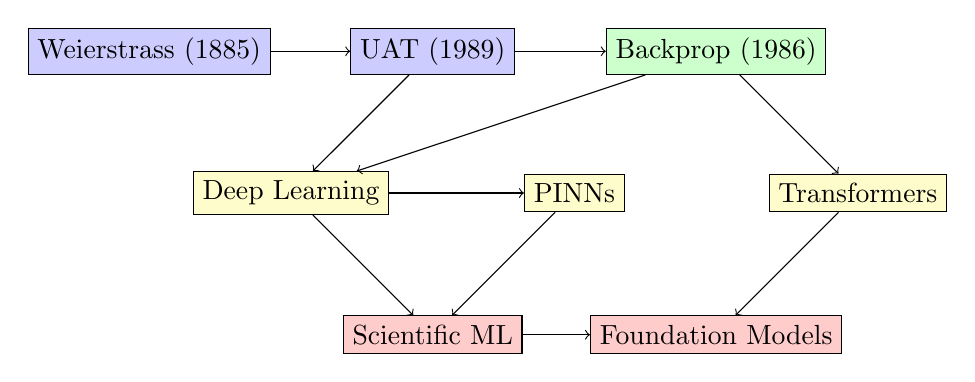
\begin{tikzpicture}[scale=0.9]
    % Historical
    \node[draw, rectangle, fill=blue!20] (w) at (0,3) {Weierstrass (1885)};
    \node[draw, rectangle, fill=blue!20] (u) at (4,3) {UAT (1989)};
    \node[draw, rectangle, fill=green!20] (b) at (8,3) {Backprop (1986)};
    
    % Modern
    \node[draw, rectangle, fill=yellow!20] (d) at (2,1) {Deep Learning};
    \node[draw, rectangle, fill=yellow!20] (p) at (6,1) {PINNs};
    \node[draw, rectangle, fill=yellow!20] (t) at (10,1) {Transformers};
    
    % Future
    \node[draw, rectangle, fill=red!20] (s) at (4,-1) {Scientific ML};
    \node[draw, rectangle, fill=red!20] (f) at (8,-1) {Foundation Models};
    
    % Connections
    \draw[->] (w) -- (u);
    \draw[->] (u) -- (b);
    \draw[->] (u) -- (d);
    \draw[->] (b) -- (d);
    \draw[->] (d) -- (p);
    \draw[->] (b) -- (t);
    \draw[->] (d) -- (s);
    \draw[->] (p) -- (s);
    \draw[->] (t) -- (f);
    \draw[->] (s) -- (f);
\end{tikzpicture}
\end{center}

\vspace{0.5cm}

\textbf{Current frontiers:}
\begin{itemize}
    \item Neural operators for PDEs
    \item Geometric deep learning
    \item Equivariant networks
    \item Uncertainty quantification
    \item Multi-scale methods
\end{itemize}
\end{frame}

\begin{frame}{Summary}
\begin{center}
\Large{We've journeyed from Weierstrass to modern deep learning}
\end{center}

\vspace{0.5cm}

\textbf{Key insights:}
\begin{itemize}
    \item Neural networks provide a universal, flexible function approximation framework
    \item Mathematical foundations (UAT) guarantee approximation capabilities
    \item Nonlinearity + depth = expressivity
    \item Automatic differentiation enables efficient training
    \item Applications span from simple classification to solving PDEs
\end{itemize}

\vspace{0.5cm}

\textbf{For Scientific ML:}
\begin{itemize}
    \item Mesh-free PDE solvers
    \item Data-driven discovery
    \item Multi-physics modeling
    \item Uncertainty quantification
\end{itemize}

\vspace{0.5cm}

\begin{center}
\textbf{The universal approximation theorem tells us neural networks CAN work. \\
Backpropagation tells us HOW to make them work.}
\end{center}
\end{frame}

\begin{frame}
\begin{center}
\Huge{Questions?}

\vspace{1cm}

\large{Thank you!}

\vspace{1cm}

\normalsize{
krishnak@utexas.edu \\
\url{https://github.com/kks32-courses/sciml}
}
\end{center}
\end{frame}

\end{document}